\chapter{Methods}\label{chap:methods}
% Evaluation Criteria:
% - Explanation
% - Reproducibility
% - Visualization
\todo{write methods introduction}
{\color{blue}
Chapter on tools (language models) used. What exactly do I want to explain?
First, a bit on how they work in general, second a bit of background on the models, a bit of a comparison (architecture and benchmarks?)
}

% background is more general, methods is specific to the methods we use, in our case LLMs

\section{Language Model Basics}\label{sec:basics}
This Section aims to provide an overview and fundamental understanding of the underlying concepts and terminology of the language models used in this work.
The models part of the benchmark are introduced in \secref{models}.
We will first establish the fundamentals of the transformer architecture in \subref{transformer} and take a look at the development to a \acrlong{LLM} in \subref{llm} before combining a number of common adaptions to visualize how a modern transformer architecture often looks like in \subref{modern}.
\todo{rewrite methods basics referecing when the other parts are finished}


\subsection{The Transformer Architecture}\label{sub:transformer}
\begin{figure}[!htb]
    \begin{centering}
        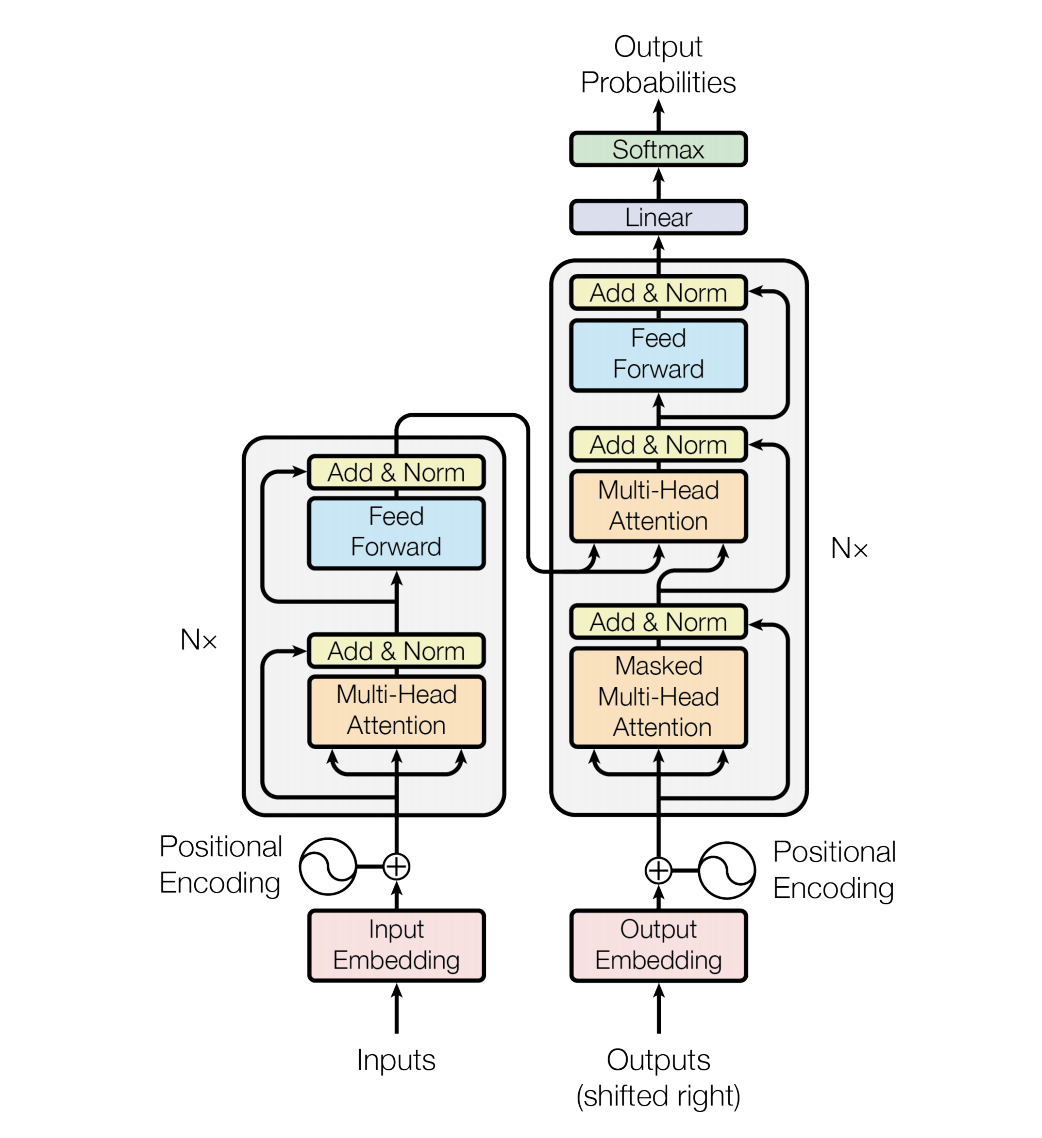
\includegraphics[height=0.5\textheight]{img/transformer}
        \caption[Original Transformer Architecture]{\textbf{Original Transformer Architecture.}
        The architecture was originally conceptualized for translation between languages.
        For that effect the text to translate (input) will be fully encoded to the embedding space, added to a positional encoding, and passed through alternating layers of self-attention and \gls{MLP} feed-forward layers with \gls{ReLU} activation, with residual connections and normalization after each.
        Output is generated autoregressively (generating each output token one-by-one, and append it to outputs to generate the next one), and has an additional layer of cross-attention to the input embedding.
        \Glspl{causal} are exclusively autoregressive decoder-only models.
        % The text to translate \textit{from} is the input, and the model will autoregressively (append selected output token to the outputs to generate the next output token until the full output has been generated) generate the full output.
        Image Source: \cite{vaswani_attention_2017}
        }
        \label{fig:transformer}
    \end{centering}
\end{figure}

% \begin{figure}[!htbp]
%     \begin{centering}
%         \subfloat[Runtime in minutes for correcting 25kb Matrix]
%         {\includegraphics[scale=0.9]{figures/results/runtime_25}} \\
%         % \caption[Correction time of 25kb]
%         % {\textbf{Runtime in minutes} for correcting the 25kb matrix.}
%         \subfloat[Runtime in minutes for correcting 50kb Matrix]
%         {\includegraphics[scale=0.9]{figures/results/runtime_50}}
%         \caption[Algorithm Runtimes]
%         {\textbf{Algorithm Runtimes} for correcting the different matrices. It
%         remains an open question why the difference between KR and RUST stays the
%         same, even though both ICE and RUST double their computation time. Smaller
%         is better.}
%         \label{fig:transformer}
%     \end{centering}
% \end{figure}

All modern language models are based on what Google introduced as the transformer architecture \cite{vaswani_attention_2017} in 2017, see the caption in \figref{transformer} for a more detailed description.
\todo{actually include parts on the encoder and decoder in text here. Don't just rely on the figure description}
This new transformer architecture quickly established itself by outperforming other architectures available at the time with a fraction of the training cost.
An Encoder-Only transformer architecture, specifically \gls{BERT} set a new \gls{SOTA} for all \gls{NLP} benchmarks established at the time.

In 2019 \gls{OpenAI} introduced \gls{GPT2} \cite{radford_language_2019}, a very straightforward transformer architecture but scaled up more than previous models. \gls{GPT2} mainly demonstrated that bigger \glspl{LM} get more capable in general.
\todo{kinda reads more like a history book}
The biggest \gls{GPT2} variant had 1.5 billion parameters, which is 15x more parameters than the biggest \gls{BERT} variant had.
Others introduced models with similar parameter counts and capabilities.
\todo{figure out final main point I want to make}
% Along with significantly increasing capability in \acrlong{NLP}, these models enabled more sophisticated requests for data extraction.

% main difference to before: enabled more context compared to LSTM-based attention stuff (andscaling)

\subsection{Large Language Models}\label{sub:llm}
Models with more than a few billion parameters became generally referred to as a \acrlong{LLM}. \gls{GPT3}, the first such model with 176 billion parameters was introduced by \gls{OpenAI} in 2020 \cite{brown_language_2020}.
\glspl{LLM} differ from previous models in both parameter count (usually many billions) and substantial advances in general capability.
These models tend to have smaller siblings of the same architecture with fewer parameters, commonly in th steps of 7 billion, 13 billion, 30 billion, and 70 billion, though availability and exact parameter count varies.
Other Organisations trained \glspl{LLM} of this generation as well, some of them open-source, which demonstrated similar capabilities.
The most well-known models of this wave were \model{BLOOM} and \model{OPT} (throughout 2022).

The most recent and most capable generation of \glspl{LM} got introduced starting early 2023, after the release of \gls{ChatGPT} sparked worldwide interest in \glspl{LLM}. Progress happened fast and many incorporated numerous of the collectively found possible improvements. \glspl{LLM} of this generation are mostly classified so by their capability, and less so through parameter size, albeit their parameter counts still tend to be in the dozens of billions. Models of this category include the open-source \model{llama} and its well-known derivatives \model{alpaca} and \model{vicuna}, \model{falcon}, as well as most recently \model{llama2}.

For more details on most of the aforementioned models, see \secref{models}.

\subsection{The Modern Transformer Architecture}\label{sub:modern}
See \figref{modern_transformer}.
\todo{rewrite subsection on modern transformer}

Over time, people figured stuff out. We have some explanations for why something works better, but most of it is still only speculation, and has been proven empirically more so than theoretically. 
One of the first things they found was that using SwiGLU as activation function instead of ReLU improved results. \todo{glossary / acronym entries for ReLU, SwiGLU, MLP?}
Instead of the previous sinusoidal positional encoding, they figured out that using \gls{RoPE} worked a lot better.
Also, normalization before, not after each sub-layer works a lot better.
As well as grouping some of the query heads for \gls{GQA}. This reduced parameters, speeds up evaluation and training, and delivers better results overall.
\begin{figure}[!htbp]
    \begin{centering}
        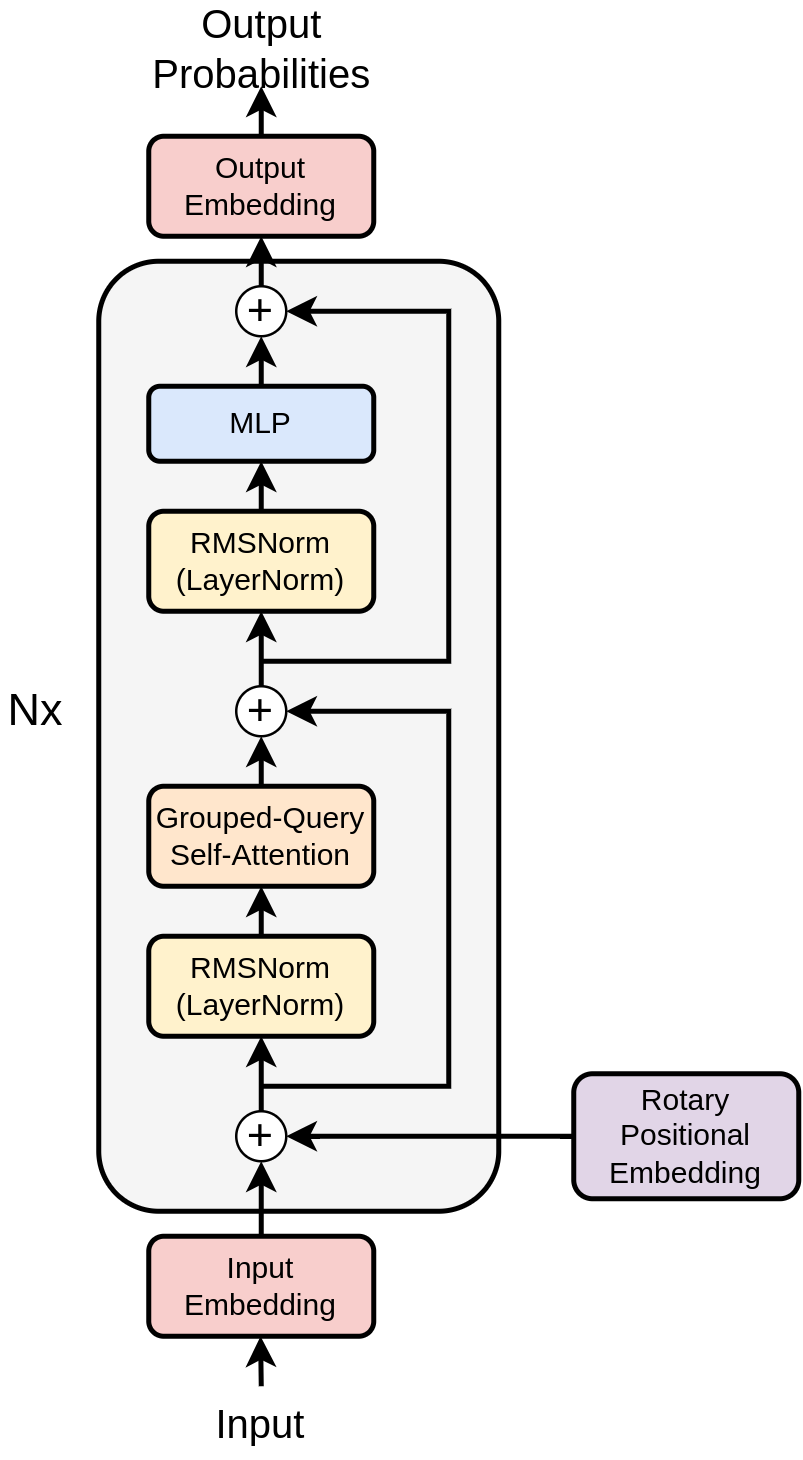
\includegraphics[height=0.8\textheight]{img/modern_transformer}
        \caption[Example of a Modern Transformer Architecture]{\textbf{Example of a Modern Transformer Architecture.} There are a number of differences when compared to the original architecture as seen previously in \figref{transformer}: layers are normalizing the residual with RMSNorm instead of having a normalized residual. Multi-head attention got replaced with \gls{GQA}, and sinusoidal positional embeddings with embeddings from \gls{RoPE} {\em on each layer}. Additionally, activation functions in the \gls{MLP} changed from \gls{ReLU} to \gls{SwiGLU}.}
        \label{fig:modern_transformer}
    \end{centering}
\end{figure}



\section{Training Methods}\label{sec:training}
\todo{write section on training methods}

\subsection{Pretraining}\label{sub:pretraining}
for main training usually crossentropy loss on text, decent batchsizes, large scale distributed.
\todo{write subsection on pretraining}

\subsection{Fine-Tuning}\label{sub:finetune}
specialized, mostly task-specific training making use of transfer-learning from a generalized model, making them capable for tasks where not much data is available
\todo{write subsection on finetuning}

\subsection{Fine-Tuning on Instructions}\label{sub:instruct}
mostly just changing 'expectation distribution' of model, giving preferred answers when interacting with the model for most people

a model fine-tuned on a instruction dataset or setting is commonly referred to as a 'instruct'-variant.
\todo{write subsection on instruction-finetuning}

\subsection{RLHF}\label{sub:rlhf}
learning preference policy to later fine-tune the large model on. basically lobotomization, as it drastically reduces capability.
Well, write it a bit nicer than that.
\todo{this is not really relevant for my thesis. remove? or write?}
